\section{Evaluation}
\label{sec:eval}

% 评估章节：Setup → 整体对比 → 稀疏感知分配器隔离实验 →
% 邻居估算敏感性 → 跨规模 → 延迟 → takeaways。

\subsection{Setup}
\label{sec:setup}

\textbf{Constellation.} Our main testbed is a Starlink Shell-1 Walker
constellation~\cite{giuliari2020} interconnected in a $+$Grid pattern
(\cref{tab:constellation}); orbital dynamics are derived from the
Satellite Tool Kit (STK). With 1{,}584 satellites, an average path length
of 23.51 hops, and a diameter of 47, capacity conflicts between demands
are far more frequent than in the terrestrial WANs used in prior TE
studies~\cite{teal}. For the cross-scale check
(\cref{sec:cross-scale}) we use a one-third-scale instance of the same
architecture (24 planes $\times$ 22 satellites, 528 nodes).

\begin{table}[t]
    \caption{Simulation parameters of the Starlink constellation.}
    \label{tab:constellation}
    \centering
    \footnotesize
    \begin{tabular}{@{}ll@{}}
        \toprule
        Parameter & Value \\
        \midrule
        Height of LEO satellites & 550 km \\
        Constellation configuration & Walker \\
        Total number of satellites & 1{,}584 \\
        Number of orbital planes & 72 \\
        Satellites per plane & 22 \\
        Inclination of orbits & $55^{\circ}$ \\
        Phase factor & 3 \\
        Inter-satellite links & 6{,}336 \\
        \bottomrule
    \end{tabular}
\end{table}

\textbf{Traffic.} Traffic matrices are generated by random city
sampling~\cite{giuliari2021}: cities are drawn with probability
proportional to their population, each sampled city pair is attached to
its nearest satellites, and per-pair flows are aggregated into
satellite-level demands (\cref{tab:tm-stats}). We use 101 consecutive
snapshots (one every 5 minutes), with snapshots 0--79 for training,
80--89 for validation, and 90--100 for testing, a strict temporal
split with no leakage. Under the chosen ISL capacities, a path-restricted
LP with complete traffic information attains a mean MLU of
${\approx}1.38$ on the test snapshots. The main setting therefore tests load
balancing under overload, not guaranteed capacity-feasible delivery;
\cref{sec:complete-te} defines the meaning of MLU above one. Demand pruning (\cref{sec:scaling})
restricts the modeled
demand set to the ${\sim}6.3$K pairs that ever carry traffic, out of
2.5M node pairs.

\begin{table}[t]
    \caption{Statistics of the population-based traffic trace (Mbps).}
    \label{tab:tm-stats}
    \centering
    \footnotesize
    \setlength{\tabcolsep}{4pt}
    \begin{tabular}{@{}lc@{}}
        \toprule
        Metric & Value \\
        \midrule
        Snapshots (5-min interval) & 101 \\
        Nonzero demand, max & 1{,}800 \\
        Nonzero demand, mean$\pm$std & 159.5 $\pm$ 242.3 \\
        Total demand per snapshot & 890{,}242 \\
        Active pairs per snapshot & 5{,}583 \\
        Active-pair union (trace) & 6{,}334 \\
        \bottomrule
    \end{tabular}
\end{table}

\textbf{Metric and protocol.} Our metric is the \emph{realized MLU}
evaluated against ground-truth demands (lower is better); flow
conservation in \cref{eq:conserve} is enforced by construction, so MLU
cannot be gamed by under-serving traffic. We sweep the observation
ratio $\rho \in \{0.02, 0.05, 0.1, 0.3, 0.5\}$ and use five independent
experimental repeats per configuration, controlled by random seeds
0--4. Matching repeat indices use the same seed across methods. Unless
stated otherwise, every method is paired with the \emph{identical deployable
post-processing layer}: two rounds of ten rebalancing sweeps, whose
utilization estimate reads only the sparse observation with neighbor fill
(\textsc{obs-nbr}, \cref{sec:training}),
so that no method receives unavailable demand information and the
allocator remains the only factor that varies. The \textsc{oracle} variant,
which reads the ground-truth matrix, appears only in the neighbor-estimation
diagnostic. Each plotted point is the mean MLU over the same eleven
chronological test snapshots for one experimental repeat. We show all five
repeats and summarize them by mean$\pm$standard deviation, median, and range.
Because the snapshots in a trace are temporally correlated, headline
comparisons are paired on $(\rho,\text{repeat})$, not on snapshots, and are
assessed with two-sided sign tests.

\textbf{Baselines.} All learned baselines share the training pipeline,
path sets, and optional neighbor-assisted refinement of \sysname{} and differ
only in how they handle sparsity:
\begin{itemize}
    \item \emph{zero-fill}: the sparse adaptation of full-observation
    systems such as Teal~\cite{teal} and SaTE~\cite{sate}, which
    cannot run on an incomplete matrix; unobserved entries are set to
    zero and the model is trained end to end on the filled input.
    SaTE's heterogeneous-graph allocator targets the same
    MLU objective with the same pruning, so this variant is its
    closest sparse-input proxy.
    \item \emph{mean-interp}: a two-stage complete-then-optimize
    baseline that fills unobserved entries with the mean of observed
    demands before allocation.
    \item \emph{nbr-fill}: a stronger two-stage baseline that fills
    each unobserved demand from observed demands sharing its source
    satellite, the same estimate used by the optional refinement.
    \item \emph{TEST-inspired}: a controlled baseline motivated by
    TEST~\cite{test}, with zero-filled input, a Transformer over the
    observation history ($L=3$), and an ungated GCN. We use the same paths,
    objective, and training pipeline as the other methods rather than
    claiming reproduction of TEST's original terrestrial setup.
    \item \emph{untrained}: the \sysname{} architecture with weights
    frozen at random initialization, isolating the contribution of
    training. It is \emph{not} the LP optimum: the LP (\cref{eq:mlu}) needs
    the complete matrix and serves only as a full-information lower-bound
    reference for MLU (${\approx}1.38$), not as an online sparse-input baseline.
\end{itemize}

\begin{table}[t]
    \caption{Model and training hyperparameters (defaults held fixed
    across all $\rho$ and repeats).}
    \label{tab:hparams}
    \centering
    \footnotesize
    \setlength{\tabcolsep}{4pt}
    \begin{tabular}{@{}ll@{}}
        \toprule
        Parameter & Value \\
        \midrule
        FlowGNN layers $\Lambda$ & 6 \\
        Candidate paths $\kappa$ & 4 \\
        Temporal $d_{\mathrm{model}}$ / heads / layers & 16 / 2 / 1 \\
        Fusion dim $d_{\mathrm{fuse}}$ & 8 \\
        History length $L$ & 3 \\
        COMA samples per update & 30 \\
        Mask-embedding init & 57.0 (median nonzero demand) \\
        \midrule
        Learning rate & $1\!\times\!10^{-4}$ \\
        Epochs (warmup / early stop) & 60 (4 / on) \\
        Restart screening & 3 inits \\
        Batch size & 20 \\
        Untrained control & 0 epochs, 1 init \\
        Neighbor refinement (deployed) & 2 rounds $\times$ 10 sweeps \\
        \midrule
        Trainable parameters & 4{,}468 \\
        \bottomrule
    \end{tabular}
\end{table}

\textbf{Implementation.} \Cref{tab:hparams} lists the
hyperparameters, drawn from the code defaults and held fixed across all
$\rho$ and repeats. The untrained control shares the trained model's
random initialization and differs only in skipping gradient updates
(\texttt{epochs${=}0$}); it is therefore a clean ablation of the
\emph{training} factor with identical architecture, mask embedding, and
post-processing.

\subsection{Performance of \sysname{}}
\label{sec:own-results}

Across observation ratios from $2\%$ to $50\%$, \sysname{} achieves a
mean realized MLU in the $1.64$--$1.89$ range (the \sysname{} row of
\cref{tab:overall}), tightening as more demands become visible: from $1.885$
at $\rho=0.05$ down to $1.639$ at $\rho=0.5$. To calibrate these numbers we
solve a path-restricted LP that sees the \emph{complete} matrix on the same
test snapshots and candidate paths; it attains a full-information optimum of
MLU~${\approx}1.38$. Observing only a fraction of demands, \sysname{} stays
within $1.19$--$1.37\times$ of this optimum. An MLU of $1.7$ means that the
assigned load on the busiest link is $70\%$ above its capacity. Flow
conservation is maintained, but capacity feasibility is not: the metric
does not imply that all offered traffic is delivered within the epoch.
These overloaded-load-balancing results cannot establish delay, loss, or
admission-control guarantees. The full-observation LP provides a lower bound
on achievable MLU for the chosen paths, not an online sparse-input baseline;
it is distinct from the \emph{untrained} control, which uses random weights.

\subsubsection{Inference latency}
\label{sec:runtime}
On the 1{,}584-satellite constellation, one complete allocation pass
(demand-set assembly, graph rebuild, gated GNN, temporal encoder, fusion,
policy head, and optional neighbor-assisted refinement) completes in under
$0.4$~s per snapshot on a single GPU, against a 5-minute control period.
Combined with the $O(D)$ complexity of \cref{sec:complexity} and the
4{,}468-parameter model size, \sysname{} fits the compute envelope of a
constellation controller.

\subsubsection{Cross-scale generality}
\label{sec:cross-scale}
To test whether the allocator depends on constellation scale, we reuse its
size-invariant architecture on a one-third-scale Shell-1 instance with 528
satellites and 2{,}112 ISLs. \Cref{tab:cross-scale} isolates the learned
allocation prior without post-processing at two observation ratios. At
$\rho=0.05$, training lowers median MLU from $4.02$ to $3.04$ and improves all
three matched repeats. The result at $\rho=0.3$ is mixed, indicating that the
most informative observation regime shifts with traffic density. The model
requires no architectural change as the graph and demand-set sizes change,
which supports reuse across constellation scales while avoiding a claim of
uniform gains.

\begin{table}[t]
    \caption{Cross-scale check on the 528-satellite instance without
    post-processing (median MLU and paired training gain over three repeats).}
    \label{tab:cross-scale}
    \centering
    \footnotesize
    \setlength{\tabcolsep}{4pt}
    \begin{tabular}{@{}lcccc@{}}
        \toprule
        $\rho$ & Trained & Untrained & Paired gain & \sysname{} lower \\
        \midrule
        0.3  & 3.69 & 3.83 & $-3.2\%$  & 1/3 \\
        0.05 & 3.04 & 4.02 & $+24.4\%$ & 3/3 \\
        \bottomrule
    \end{tabular}
\end{table}

\subsection{Comparison with Sparsity Treatments}
\label{sec:overall}

We now compare \sysname{} against external sparsity treatments under the
identical deployable protocol. \Cref{fig:overall-distribution} shows all
150 results from repeated runs, while \cref{tab:overall} gives their numerical
summary. No method has a uniform advantage across observation ratios. In
particular, \sysname{} attains a lower MLU than zero filling on 16 of the 25
matched $(\rho,\text{repeat})$ pairs, but the paired sign test gives
$p=0.2295$; its comparisons with TEST-inspired, mean-interp, nbr-fill, and
untrained controls are likewise non-significant (\cref{tab:paired}). Hence
the observed rankings must be interpreted together with their variability;
they do not establish overall superiority.

\begin{figure*}[t]
    \centering
    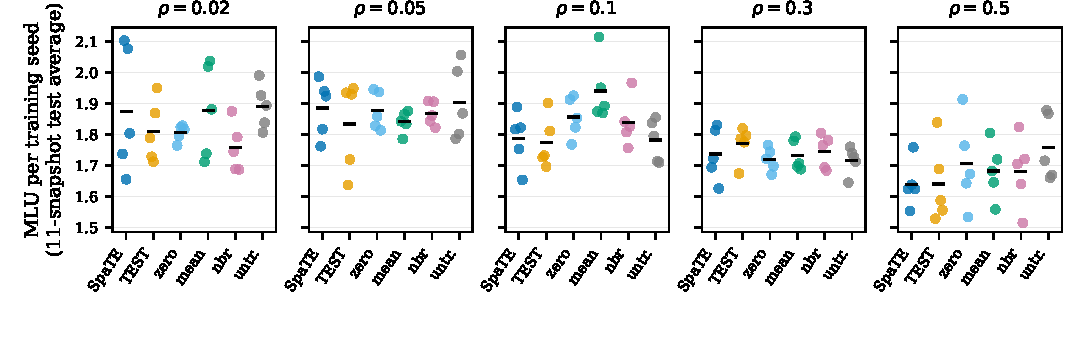
\includegraphics[width=\textwidth]{figs/overall_distribution.pdf}
    \caption{External comparison across five experimental repeats under
    the same deployed neighbor-assisted refinement. Each marker is one
    repeat's average MLU over
    the 11 test snapshots; black bars mark means. The dispersion explains why
    column-wise rankings based only on a median are not reliable evidence of
    a general advantage.}
    \label{fig:overall-distribution}
\end{figure*}

\begin{table*}[t]
    \caption{External comparison under the aligned deployable protocol.
    Entries are mean$\pm$standard deviation across five experimental repeats;
    medians and ranges are included in the supplementary CSV. Lower MLU is
    better.}
    \label{tab:overall}
    \centering
    \scriptsize
    \setlength{\tabcolsep}{5pt}
    \begin{tabular}{@{}lccccc@{}}
        \toprule
        & \multicolumn{5}{c}{observation ratio $\rho$} \\
        \cmidrule(lr){2-6}
        Method & 0.02 & 0.05 & 0.1 & 0.3 & 0.5 \\
        \midrule
        \sysname{} & $1.874\pm0.203$ & $1.885\pm0.093$ & $1.786\pm0.089$ & $1.737\pm0.085$ & $1.639\pm0.074$ \\
        TEST-inspired~\cite{test} & $1.809\pm0.100$ & $1.833\pm0.145$ & $1.773\pm0.083$ & $1.769\pm0.056$ & $1.639\pm0.127$ \\
        zero-fill~\cite{teal,sate} & $1.805\pm0.026$ & $1.876\pm0.061$ & $1.856\pm0.065$ & $1.719\pm0.038$ & $1.705\pm0.142$ \\
        mean-interp & $1.877\pm0.152$ & $1.840\pm0.035$ & $1.939\pm0.103$ & $1.732\pm0.050$ & $1.682\pm0.091$ \\
        nbr-fill & $1.756\pm0.079$ & $1.867\pm0.038$ & $1.839\pm0.078$ & $1.745\pm0.054$ & $1.680\pm0.114$ \\
        untrained & $1.890\pm0.073$ & $1.902\pm0.121$ & $1.781\pm0.068$ & $1.716\pm0.044$ & $1.757\pm0.107$ \\
        \bottomrule
    \end{tabular}
\end{table*}

\begin{table}[t]
    \caption{Paired comparison of \sysname{} against each external control
    over 25 $(\rho,\text{repeat})$ pairs. The middle column counts the pairs in
    which \sysname{} attains the lower MLU (out of 25); there are no ties.
    $p$ is a two-sided sign test.}
    \label{tab:paired}
    \centering
    \footnotesize
    \setlength{\tabcolsep}{4pt}
    \begin{tabular}{@{}lcc@{}}
        \toprule
        Control & \sysname{} lower / 25 & $p$ \\
        \midrule
        TEST-inspired & 11 & 0.6900 \\
        zero-fill & 16 & 0.2295 \\
        mean-interp & 16 & 0.2295 \\
        nbr-fill & 15 & 0.4244 \\
        untrained & 14 & 0.6900 \\
        \bottomrule
    \end{tabular}
\end{table}

\subsection{Ablations}
\label{sec:allocator-isolation}

\subsubsection{Effect of training}
We isolate the contribution of training by comparing \sysname{} with its
untrained counterpart under the common neighbor-assisted refinement.
\Cref{fig:internal-training} plots the five test averages for each condition,
one per experimental repeat.
Training attains the lower MLU in 14 of the 25 matched $(\rho,\text{repeat})$
pairs and the higher in 11, with no ties (two-sided sign test $p=0.690$). At
$\rho=0.5$, for example, the mean is $1.639\pm0.074$ after training versus
$1.757\pm0.107$ without training; at the other ratios the paired outcomes are
mixed. Thus these data do not establish a statistically significant
end-to-end training advantage, but they expose the initialization sensitivity that a
single aggregate score would hide.

\begin{figure*}[t]
    \centering
    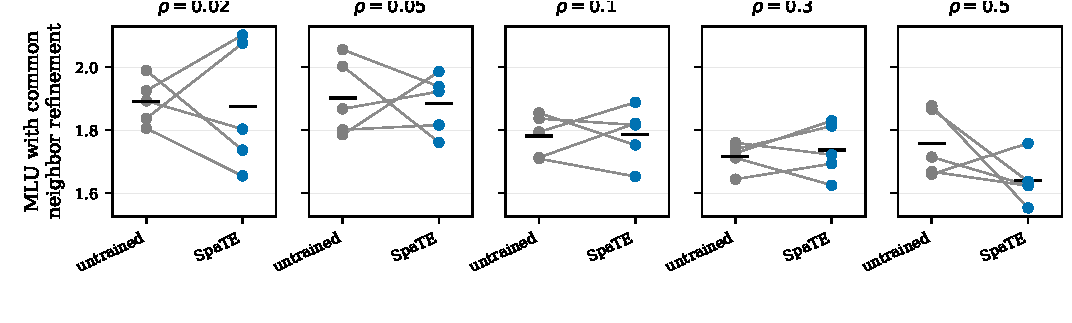
\includegraphics[width=\textwidth]{figs/internal_training.pdf}
    \caption{Effect of training under identical neighbor-assisted refinement.
    Gray dots denote the untrained control and blue dots denote \sysname{}.
    Each dot is one repeat's mean MLU over the same 11 test snapshots; slight
    horizontal offsets distinguish the five repeats, and black bars mark
    their means. Matching repeats share a random seed; no connecting lines
    are drawn.}
    \label{fig:internal-training}
\end{figure*}

\subsubsection{Representation components}
We next test the three representation choices without post-processing at the
two sparsest ratios, where their effect is least likely to be hidden by
rebalancing. \Cref{fig:component-lowrho} shows each experimental repeat. The
outcomes are mixed: no configuration dominates the others at both ratios,
and the three-repeat diagnostic is insufficient for a component-level
performance claim. We therefore retain the placeholder-isolation result of
\cref{prop:isolation} as a structural property, rather than interpreting it
as proof that gating, masking, or temporal encoding always lowers MLU.

\begin{figure*}[t]
    \centering
    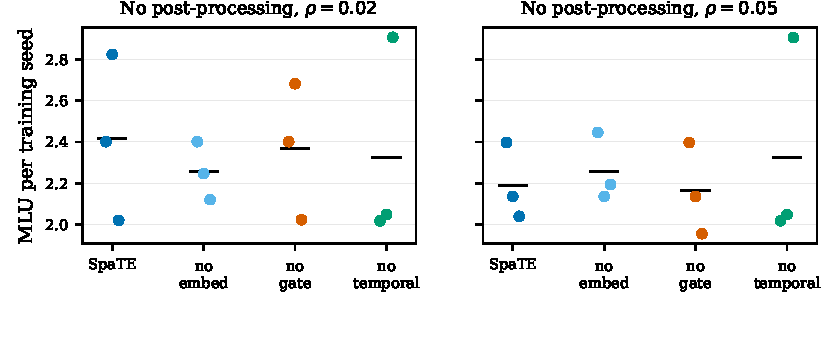
\includegraphics[width=0.76\textwidth]{figs/component_lowrho.pdf}
    \caption{Low-observability component diagnostic without post-processing
    (three experimental repeats). Dots are test averages from individual
    repeats and black bars are means. The mixed ordering supports treating
    the module choices as design alternatives rather than assuming a uniform
    component gain.}
    \label{fig:component-lowrho}
\end{figure*}

\subsubsection{Sensitivity to the neighbor estimate}
\label{sec:neighbor-estimate}
The optional refinement pass needs an estimated traffic matrix only to rank
candidate paths by congestion. \Cref{fig:neighbor-ladder} fixes the
untrained control at $\rho=0.3$ and shows all three experimental repeats.
Moving from no post-processing (median $2.833$) to an observation with zeros
elsewhere ($2.295$), and then to the source-neighbor estimate ($1.740$),
substantially changes the congestion signal available to the rebalancer. The
oracle reference reaches $1.599$, but uses unavailable ground-truth traffic
and five rounds of ten sweeps; it is a full-information diagnostic rather
than a protocol-matched baseline. The deployable conclusion is therefore limited to the value of the
neighbor estimate over zero filling, not a claim that post-processing is the
central learned mechanism.

\begin{figure}[t]
    \centering
    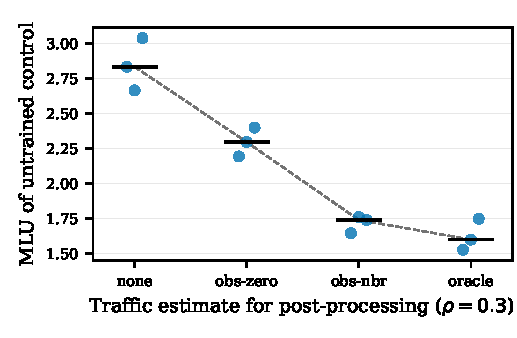
\includegraphics[width=\linewidth]{figs/neighbor_ladder.pdf}
    \caption{Sensitivity to the traffic estimate used by post-processing at
    $\rho=0.3$. Each dot is one experimental repeat; black bars denote medians.
    The oracle uses unavailable complete traffic and five rounds of ten
    sweeps; deployed methods use an observation-derived estimate.}
    \label{fig:neighbor-ladder}
\end{figure}

\subsection{Takeaways}
\label{sec:takeaways}

\begin{itemize}
    \item The distribution across experimental repeats, not a column-wise
    median, is required to interpret sparse-observation TE: none of \sysname{}'s
    external pairwise comparisons is statistically significant.
    \item Training and the three representation choices show mixed outcomes
    in the available internal diagnostics; the architecture's structural
    properties should not be read as a universal performance guarantee.
    \item Source-neighbor estimation provides a substantially more useful
    deployable congestion signal than zero filling in the $\rho=0.3$
    diagnostic, while the oracle remains an unavailable reference.
\end{itemize}
